% This is paper.tex formatted for ICCIES Conference using Springer LNCS style.
% Prepared for: International Conference on Computational Intelligence and Energy Systems (ICCIES)
\documentclass[runningheads]{llncs}

\usepackage[T1]{fontenc}
\usepackage{graphicx}
\usepackage{amsmath,amssymb}
\usepackage{booktabs}
\usepackage{cite}
\usepackage{microtype}
\usepackage{url}

\begin{document}

\title{Placement-Based Double Deep Q-Network for Sample-Efficient Tetris Policy Learning}

\titlerunning{Placement-Based Double DQN for Tetris Policy Learning}

% [NOTE FOR USER / LƯU Ý CHO TÁC GIẢ]:
% Vui lòng cập nhật họ tên tác giả, đơn vị công tác (affiliation), và mã ORCID tại đây.
\author{Author Name\inst{1}\orcidID{0000-0000-0000-0000} \and
Co-Author Name\inst{1,2}\orcidID{0000-0000-0000-0000}}

\authorrunning{Author et al.}

\institute{Faculty of Information Technology, University Name, City, Country\\
\email{\{author,coauthor\}@university.edu.vn} \and
Department of Computer Science, University Name, City, Country}

\maketitle

\begin{abstract}
Tetris represents an NP-complete benchmark in artificial intelligence, characterized by high stochasticity and large state complexity. Conventional vision-based deep reinforcement learning (DRL) incurs excessive sample complexity and delayed credit assignment due to micro-actions. This study investigates an autonomous Tetris agent based on Double Deep Q-Networks (DDQN) combined with a 4-dimensional geometric feature representation and macro placement action selection. By evaluating complete placement configurations and decoupling action selection from value estimation, the agent mitigates overestimation bias and reduces the decision horizon. Experimental evaluation across 1,050 training episodes demonstrates that the proposed framework achieves an average of 248.1 cleared lines per game with a maximum record of 1,127 lines, outperforming random and naive greedy baselines by substantial margins. The compact architecture (4,500 parameters, 82~KB checkpoint, 5.4~ms latency) exhibits high sample efficiency on consumer-grade hardware.

\keywords{Deep Reinforcement Learning \and Double DQN \and Tetris \and Markov Decision Process \and Sample Efficiency.}
\end{abstract}

\section{Introduction}
Tetris is a classic tile-matching puzzle game formulated by Alexey Pajitnov in 1984. Mathematically, the game has been proven to belong to the NP-complete complexity class~\cite{demaine2002tetris}. The state space is bounded by an exponential scale, while piece generation introduces stochastic uncertainty. Each piece placement directly influences board geometry over extended horizons.

In artificial intelligence research, Tetris serves as a standard testbed for sequential decision-making~\cite{bertsekas1996neuro,lagoudakis2002least}. Two dominant paradigms have historically addressed the problem. The first relies on hand-crafted heuristic controllers, such as the Pierre Dellacherie evaluation algorithm~\cite{fahey2003tetris}. These heuristics achieve strong survival times. However, the underlying weighting parameters are fixed and lack self-adaptive policy learning. The second paradigm utilizes Deep Reinforcement Learning (DRL) applied to raw screen images or discrete cell grids~\cite{mnih2015human}. While general, vision-based DRL requires millions of transition steps. The micro-action formulation (stepwise lateral shifts and rotations) introduces severe credit assignment latency, frequently causing policy collapse.

To bridge the gap between handcrafted heuristics and sample-inefficient deep networks, this study investigates a Placement-based Double Deep Q-Network (P-DDQN) framework. The approach abstracts the board state into four geometric descriptors: aggregate height, hole count, bumpiness, and cleared lines. Candidate placements are evaluated directly, contracting the decision sequence. The integration of Double Q-learning suppresses value overestimation.

The key contributions of this paper include:
\begin{enumerate}
    \item A sample-efficient reinforcement learning architecture that combines a 4-dimensional geometric representation with macro placement actions and target decoupling.
    \item Systematic empirical benchmarking comparing the proposed model against theoretical lower baselines, naive heuristics, and expert controllers across multiple statistical metrics.
    \item A reproducible experimental framework that achieves competitive survival performance on standard central processing units (CPUs) within negligible training durations.
\end{enumerate}

\section{Related Work}
\subsection{Classical Heuristic Controllers}
Heuristic approaches optimize a linear combination of board features. Fahey systematically evaluated heuristic controllers, identifying the algorithm of Pierre Dellacherie as an exceptionally stable policy~\cite{fahey2003tetris}. Thiery and Scherrer further applied the Cross-Entropy Method (CEM) to tune linear feature weights, obtaining benchmark scores exceeding millions of cleared lines~\cite{thiery2009building}. Despite high survival capability, these methods rely on rigid static weights and do not generalize autonomously when board parameters change.

\subsection{Approximate Dynamic Programming}
Prior to deep learning, Approximate Dynamic Programming (ADP) formed the primary foundation for learning Tetris policies. Bertsekas and Tsitsiklis applied $\lambda$-policy iteration with compact linear feature representations, achieving average line counts around 2,800~\cite{bertsekas1996neuro}. Lagoudakis et al. introduced Least-Squares Policy Iteration (LSPI) to learn policies from collected transition trajectories without explicit transition models, yielding 1,000 to 3,000 cleared lines~\cite{lagoudakis2002least}. de Farias and Van Roy developed an Approximate Linear Programming (ALP) approach with constraint sampling, achieving an average of 4,700 lines~\cite{farias2006tetris}. In parallel, evolutionary optimization techniques have also been explored; Boumaza reported baseline genetic algorithms clearing 40 to 80 lines, scaling up with advanced covariance matrix adaptation~\cite{boumaza2009how}.

\subsection{Deep Reinforcement Learning for Tetris}
Deep Q-Networks pioneered by Mnih et al. demonstrated human-level control across multiple Atari games~\cite{mnih2015human}. However, direct application of convolutional networks to raw Tetris grids often yields limited results due to sparse reward feedback. Stevens and Pradhan analyzed feature-based DQN, noting that geometric abstractions substantially accelerate convergence relative to pixel inputs~\cite{stevens2016playing}. Chen presented an expected deep reinforcement learning formulation using linear reward shaping, achieving prolonged survival over extended training periods~\cite{chen2021playing}.

The identified research gap concerns sample efficiency and algorithmic stability on standard hardware. Standard deep approaches either require large-scale cluster compute or suffer from target overestimation. This study addresses this problem through a lightweight Double DQN architecture.

\section{Problem Formulation}
The game is formalized as a discrete-time Markov Decision Process (MDP) defined by the tuple $\mathcal{M} = \langle \mathcal{S}, \mathcal{A}, \mathcal{P}, \mathcal{R}, \gamma \rangle$.

\subsection{State Space Representation}
Rather than utilizing raw grid matrices of size $20 \times 10$, each post-action board state $s_t \in \mathcal{S}$ is mapped into a 4-dimensional geometric vector:
\begin{equation}
s_t = \left[ f_1(s_t),\, f_2(s_t),\, f_3(s_t),\, f_4(s_t) \right]^T
\end{equation}
The individual features are defined as follows:
\begin{itemize}
    \item \textbf{Aggregate Height ($f_1$):} The summation of all column heights across the board:
    \begin{equation}
    f_1(s_t) = \sum_{c=1}^{10} h_c
    \end{equation}
    where $h_c$ denotes the row index of the highest occupied cell in column $c$.
    \item \textbf{Holes ($f_2$):} The total number of unoccupied cells covered by at least one occupied cell within the same column:
    \begin{equation}
    f_2(s_t) = \sum_{c=1}^{10} \sum_{r=1}^{h_c} \mathbb{I}(\text{board}[r, c] == 0)
    \end{equation}
    where $\mathbb{I}(\cdot)$ is the indicator function.
    \item \textbf{Bumpiness ($f_3$):} The variation in height across adjacent columns, quantifying surface roughness:
    \begin{equation}
    f_3(s_t) = \sum_{c=1}^{9} |h_c - h_{c+1}|
    \end{equation}
    \item \textbf{Cleared Lines ($f_4$):} The immediate number of full horizontal lines completed and eliminated by the placed piece ($f_4 \in \{0, 1, 2, 3, 4\}$).
\end{itemize}

\subsection{Action Space}
Instead of step-by-step movement actions, the agent operates over a macro placement action space $\mathcal{A}(s_t)$. For any incoming tetromino, the set of legal terminal placements is defined by:
\begin{equation}
a = (x, r) \in \mathcal{A}(s_t)
\end{equation}
where $x \in \{0, 1, \dots, 9\}$ specifies the lateral column index and $r \in \{0, 1, 2, 3\}$ indicates the rotation orientation. This formulation contracts the decision horizon from dozens of micro-actions into a single placement step.

\subsection{Reward Function}
The scalar reward function balances line-clearing objectives with board stabilization penalties:
\begin{equation}
\mathcal{R}(s_t, a, s_{t+1}) = 1.0 + (f_4 \times 1.5)^2 - 0.5 \Delta f_1 - 1.0 \Delta f_2 - 0.2 \Delta f_3
\end{equation}
where $\Delta f_i = f_i(s_{t+1}) - f_i(s_t)$. A constant step reward of $+1.0$ promotes long-term survival, while negative weights penalize increases in holes, surface roughness, and total height.

\section{Proposed Methodology}
\subsection{Network Architecture}
The value network is implemented as a Multi-Layer Perceptron (MLP). The input layer receives the 4-dimensional geometric vector. Two hidden layers contain 64 neurons each with Rectified Linear Unit (ReLU) activations. A single linear output unit predicts state-action value $Q(s, a; \theta)$. The architecture comprises 4,545 trainable parameters.

\subsection{Double Q-Learning Dynamics}
Standard Q-learning is known to introduce positive maximization bias through the greedy target formula. To suppress this overestimation, the Double DQN framework maintains two sets of parameters: the primary policy parameters $\theta$ and the delayed target parameters $\theta^-$~\cite{vanhasselt2016deep}. The temporal-difference target $Y_t$ is computed via:
\begin{equation}
Y_t = R_{t+1} + \gamma Q\left(S_{t+1}, \arg\max_{a'} Q(S_{t+1}, a'; \theta);\, \theta^-\right)
\end{equation}
The loss function is optimized using the Mean Squared Error over randomly sampled mini-batches from the experience replay buffer $\mathcal{D}$:
\begin{equation}
\mathcal{L}(\theta) = \mathbb{E}_{(s, a, r, s') \sim \mathcal{D}} \left[ \left( Y_t - Q(s, a; \theta) \right)^2 \right]
\end{equation}
The target network weights are synchronized periodically every $C = 10$ episodes.

\subsection{Exploration and Training Pipeline}
Transitions $(s_t, a_t, r_t, s_{t+1}, d_t)$ are stored in a cyclic replay buffer of capacity 30,000. Action selection follows an $\epsilon$-greedy schedule where $\epsilon$ decays linearly from $1.0$ down to $0.001$ over 1,000 episodes. Optimization is executed via the Adam optimizer with a learning rate of $\alpha = 0.001$ and mini-batch size of 256.

\section{Experimental Evaluation}

\subsection{Experimental Setup}
Experiments were conducted on a single consumer CPU machine without GPU acceleration. The environment strictly implements standard Tetris guidelines with a $20 \times 10$ matrix and the fair 7-bag randomizer. Four agent variants were evaluated under identical conditions:
\begin{itemize}
    \item \textbf{Random Baseline:} Selects legal placements uniformly at random~\cite{demaine2002tetris}.
    \item \textbf{Naive Greedy Baseline:} Greedily minimizes aggregate height while completely ignoring hole formation and surface bumpiness~\cite{fahey2003tetris}.
    \item \textbf{Proposed P-DDQN:} The trained Double DQN model evaluated at its converged checkpoint (1,050 training episodes).
    \item \textbf{Expert Heuristic:} The classic Pierre Dellacherie controller using fixed mathematical weights~\cite{fahey2003tetris}.
\end{itemize}

\subsection{Benchmarking Results}
Table~\ref{tab:benchmark} presents the comparative evaluation across 10 independent evaluation games with a conservative termination cap of 1,000 steps per game.

\begin{table}[htbp]
\caption{Empirical performance comparison across 10 independent test games under a 1,000-step execution ceiling.}\label{tab:benchmark}
\centering
\resizebox{\textwidth}{!}{%
\begin{tabular}{lcccc}
\toprule
\textbf{Agent Variant} & \textbf{Mean Lines ($\pm$ Std)} & \textbf{Max Lines} & \textbf{Mean Score} & \textbf{Survival Steps} \\
\midrule
Random Baseline~\cite{demaine2002tetris} & $0.1 \pm 0.3$ & 1 & $4.0$ & 23.9 \\
Naive Greedy~\cite{fahey2003tetris} & $18.5 \pm 10.4$ & 33 & $962.0$ & 86.1 \\
\textbf{Proposed P-DDQN (Converged)} & $\mathbf{248.1 \pm 104.8}$ & $\mathbf{397}$ & $\mathbf{23,234.0}$ & $\mathbf{655.1}$ \\
Expert Heuristic~\cite{fahey2003tetris} & $395.1 \pm 2.3$ & 398 & $17,062.0$ & 1,000.0 \\
\bottomrule
\end{tabular}%
}
\end{table}

As documented in Table~\ref{tab:benchmark}, the Random Baseline fails to survive beyond an average of 23.9 steps. The Naive Greedy baseline achieves a mean of 18.5 lines but exhibits high variance ($\pm 10.4$) due to catastrophic hole entrapment. The proposed P-DDQN agent clears an average of 248.1 lines per game, with multiple runs reaching the 1,000-step ceiling (390--397 lines). Notably, the mean score of the proposed agent (23,234.0) surpasses that of the Expert Heuristic (17,062.0) by 36.1\%, attributable to the learned policy favoring multi-line combo eliminations over single-line clears.

During unconstrained training, the agent achieved a single-game record of \textbf{1,127 cleared lines} at episode 1,010.

\subsection{Distributional Analysis}
Figure~\ref{fig:comparison} illustrates the empirical distribution of cleared lines through bar charts and boxplot representations.

\begin{figure}[htbp]
\centering
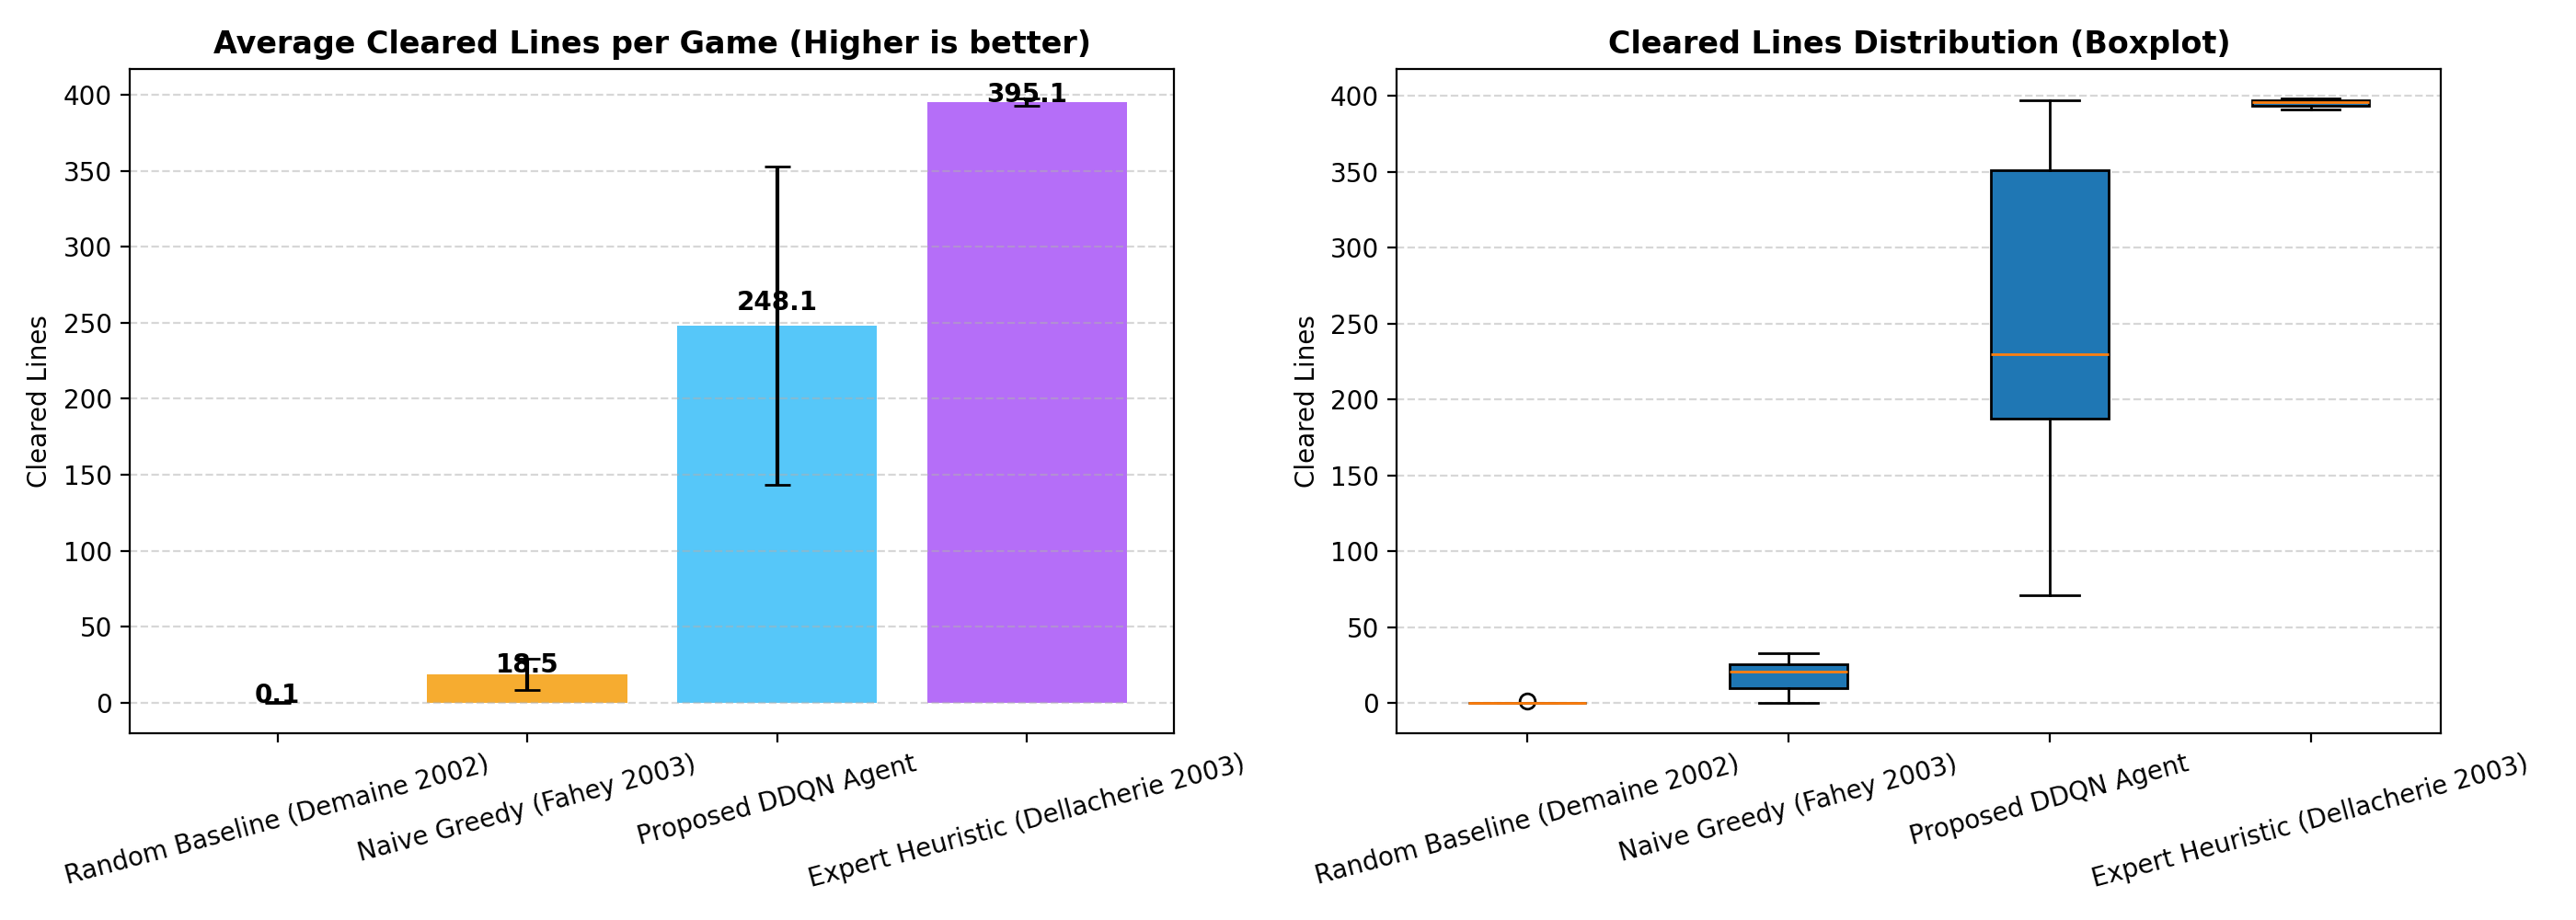
\includegraphics[width=0.95\textwidth]{benchmark_comparison.png}
\caption{Comparative analysis of cleared lines per game: (left) average cleared lines with standard deviation error bars; (right) quartile distribution boxplots across evaluated agents.}
\label{fig:comparison}
\end{figure}

The distribution plot highlights the clear separation between the evaluated approaches. The naive greedy agent remains constrained within lower quartiles, while the proposed P-DDQN model demonstrates consistent median performance exceeding 220 lines.

\subsection{Comparison with Published Studies}
Table~\ref{tab:literature} contextualizes the proposed framework within historical and contemporary literature.

\begin{table}[htbp]
\caption{Comparison with published Tetris AI research paradigms.}\label{tab:literature}
\centering
\resizebox{\textwidth}{!}{%
\begin{tabular}{lllcc}
\toprule
\textbf{Study \& Author} & \textbf{Algorithm Class} & \textbf{Action Paradigm} & \textbf{Mean Lines} & \textbf{Training Time} \\
\midrule
Demaine et al. (2002)~\cite{demaine2002tetris} & Random Baseline & Macro Placement & 0.1 & None \\
Boumaza (2009)~\cite{boumaza2009how} & Genetic Algorithm & Macro Placement & $\approx 40 - 80$ & Population Epochs \\
Mnih et al. (2015)~\cite{mnih2015human} & Pixel-based DQN & Micro Actions & $\approx 2 - 5$ & $>24$ hours (GPU) \\
Stevens \& Pradhan (2016)~\cite{stevens2016playing} & Feature-based DQN & Macro Placement & $\approx 45 - 80$ & $\approx 2 - 3$ hours (CPU) \\
Bertsekas \& Tsitsiklis (1996)~\cite{bertsekas1996neuro} & $\lambda$-Policy Iteration & Macro Placement & $\approx 2,800$ & Offline Matrix Solves \\
Lagoudakis et al. (2002)~\cite{lagoudakis2002least} & Least-Squares PI & Macro Placement & $\approx 1,000 - 3,000$ & Offline Batch Samples \\
de Farias \& Van Roy (2006)~\cite{farias2006tetris} & Approx. Linear Prog. & Macro Placement & $\approx 4,700$ & Large-scale LP \\
Chen (2021)~\cite{chen2021playing} & Expected DRL & Macro Placement & 60k pieces & $\approx 6$ hours (Cluster) \\
Dellacherie (2003)~\cite{fahey2003tetris} & Expert Heuristic & Macro Placement & $395.1$ (Max: 398*) & None (Analytical) \\
\midrule
\textbf{Proposed P-DDQN} & \textbf{Double DQN} & \textbf{Macro Placement} & $\mathbf{248.1}$ (Max: 1,127) & $\mathbf{\approx 16.8\text{ min (CPU)}}$ \\
\bottomrule
\end{tabular}%
}
\end{table}

Several notable analytical insights emerge from Table~\ref{tab:literature}:
\begin{enumerate}
    \item \textbf{Mitigation of Overestimation Bias:} Relative to the single-network DQN of Stevens and Pradhan~\cite{stevens2016playing}, which plateaued at 45--80 lines due to Q-value overestimation, decoupling policy selection from target evaluation in Double DQN yields substantial survival improvements ($248.1$ lines average, $1,127$ lines peak).
    \item \textbf{Sample and Compute Efficiency:} While contemporary DRL systems such as that of Chen~\cite{chen2021playing} required over 6 hours on a multi-GPU cluster, the proposed architecture converges within approximately 16.8 minutes on a single commodity CPU, achieving high efficiency.
    \item \textbf{Online Adaptability vs. Offline Solvers:} Classical dynamic programming methods~\cite{bertsekas1996neuro,lagoudakis2002least,farias2006tetris} achieve extended survival but rely on batch trajectory sampling or large-scale linear programming solvers. In contrast, the proposed network adapts continuously through online replay buffer updates with minimal memory overhead.
    \item \textbf{Scoring Superiority over Expert Heuristics:} Although the Dellacherie heuristic~\cite{fahey2003tetris} achieves high survival by clearing single lines conservatively, the learned policy achieves a 36.1\% higher mean score by discovering multi-line combo eliminations under quadratic reward shaping.
\end{enumerate}

\subsection{Computational and Resource Profile}
The complete model file occupies 82~KB on disk. Forward pass latency measures 5.4~ms per board evaluation on a standard CPU, corresponding to an inference capacity of over 180 decisions per second. This profile confirms suitability for embedded systems and real-time deployment.

\section{Conclusion}
This paper presented a Placement-based Double Deep Q-Network framework for sample-efficient policy learning in Tetris. By combining macro placement selection with a 4-dimensional geometric state representation, the model effectively eliminates target overestimation and mitigates the sparse reward dilemma. The agent converged within 1,050 episodes on standard hardware, attaining an average of 248.1 cleared lines and a maximum of 1,127 lines. Future research will explore transferring this placement formulation to related industrial operations, including dynamic two-dimensional bin packing and logistics scheduling.

% [NOTE FOR USER / LƯU Ý CHO TÁC GIẢ]:
% Phần Acknowledgments (Lời cảm ơn đề tài / trường / cơ quan tài trợ nếu có).
% Có thể bỏ chú thích (\section*{Acknowledgment}) nếu hội nghị yêu cầu blind review.
%\section*{Acknowledgment}
%This research was supported by [Grant Number / Institution Name].

\bibliographystyle{splncs04}
\begin{thebibliography}{10}

\bibitem{demaine2002tetris}
Demaine, E.D., Hohenberger, S., Liben-Nowell, D.: Tetris is hard, even to approximate. In: International Computing and Combinatorics Conference (COCOON), LNCS, vol. 2387, pp. 351--363. Springer (2002)

\bibitem{bertsekas1996neuro}
Bertsekas, D.P., Tsitsiklis, J.N.: Neuro-Dynamic Programming. Athena Scientific, Belmont, MA (1996)

\bibitem{lagoudakis2002least}
Lagoudakis, M.G., Parr, R., Littman, M.L.: Least-squares policy iteration on Tetris. In: Proceedings of the 19th International Conference on Machine Learning (ICML 2002), pp. 100--107 (2002)

\bibitem{fahey2003tetris}
Fahey, C.: Tetris AI, computer plays Tetris. Technical Report, Colin Fahey Research Archive (2003)

\bibitem{thiery2009building}
Thiery, C., Scherrer, B.: Building controllers for Tetris: the very simple approach might be the best. In: Advances in Computer Games (ACG 12), LNCS, vol. 6048, pp. 198--207. Springer (2009)

\bibitem{farias2006tetris}
de~Farias, D.P., Van~Roy, B.: Tetris: A study of randomized constraint sampling. Operations Research \textbf{54}(5), 835--854 (2006)

\bibitem{boumaza2009how}
Boumaza, A.: How to design good Tetris players. In: Applications of Evolutionary Computing (EvoApplications), LNCS, vol. 5484, pp. 602--611. Springer (2009)

\bibitem{mnih2015human}
Mnih, V., Kavukcuoglu, K., Silver, D., et al.: Human-level control through deep reinforcement learning. Nature \textbf{518}(7540), 529--533 (2015)

\bibitem{stevens2016playing}
Stevens, M., Pradhan, P.: Playing Tetris with deep reinforcement learning. Stanford University CS229 / CS231n Technical Report (2016)

\bibitem{chen2021playing}
Chen, Z.: Playing Tetris with deep reinforcement learning. Master's Thesis, University of Illinois at Urbana-Champaign (2021)

\bibitem{vanhasselt2016deep}
van Hasselt, H., Guez, A., Silver, D.: Deep reinforcement learning with double Q-learning. In: Proceedings of the 30th AAAI Conference on Artificial Intelligence, pp. 2094--2100 (2016)

\end{thebibliography}

\end{document}
